\documentclass[twocolumn]{article}
\usepackage{amsmath}%,mathtools}

\usepackage[margin=2cm,a4paper]{geometry}
\usepackage{subcaption,graphicx}
\usepackage{enumerate}
\usepackage{hyperref}

\title{Project Proposal\\
Word Embeddings in Multiple Languages}
\author{Sara Veldhoen \and Benno Kruit}
\date{\vspace{-5ex}}
% \date{\today}
\begin{document}
\maketitle

\section{Introduction}
The aim of our project is to obtain a single vector space that captures the semantics of many different languages at the same time. Since such a vector space is less dependent on a specific language or culture, it is supposed to be a better representation of the real world concepts underlying language. Moreover, we suspect that rare words get a more reliable representation.

Multilingual word embeddings are useful for a variety of tasks. They are already used in Machine Translation, and could prove useful for cross-lingual information retrieval, parsing and semantic frame induction.
Embedding many languages in the same means data from one language could improve word representations in other languages and mitigate sparsity.
However, this is as of yet an open research question.

%Rare words

In section~\ref{s:relatedWork} we discuss existing approaches to this task. We will reproduce these experiments for the case of more than two languages, plus a new approach that we introduce in section~\ref{s:newApproach}.

The experiments we want to conduct are explained in section~\ref{s:experiments} plus the data we plan to use. For evaluation, we will use the methods from \cite{mikolov2013exploiting,klementiev2012inducing}. We also plan to create a visualisation by mapping part of the semantic space to 2D and investigate the words in that area.




\section{Related work}\label{s:relatedWork}
Some research has focused on this problem, using both different techniques to obtain word representations, and different approaches to the cross-lingual aspects. The evaluation methods applied also vary a lot.


\subsection{Linear Mapping}\label{s:lin}

According to Mikolov et al. \cite{mikolov2013exploiting}, the vector space of word representations in different languages are geometrically similar, because words in languages are grounded in real world concepts.
It is therefore possible to find a linear mapping 
%(rotation and scaling) 
between these vector spaces.

The approach is to first train word embeddings on large monolingual data for both languages separately, using the \texttt{word2vec} implementation. In the reported experiments, the so-called CBOW architecture is used, that predicts a word given its context in both directions. 
Notably, the authors also propose a way to include some phrases: multi-word expressions. This may prove useful for translation, as one multiple words can together express a concept that has a single word in another language.

Using a relatively small set of gold standard word translations, in this case obtained from Google Translate, a transformation matrix $W$ is searched. The training objective is to minimize the distance between words that are translations of one another.

%The evaluation is performed on a test set of gold-standard word translations, again from Google Translate. The word representation in the source language is transformed using $W$, and a ranked list of the nearest words in the target language is the output. The precision at ranks 1 and 5 is reported.

% Not parallel data, but simple dictionary (Google Translate) used as gold standard. Because of this, every word has one single gold-standard translation, instead of a similarity score to several words
% Easy evaluation method = nice
% Maybe the assumption of linear translation is too strong. The interrelation of some concepts may be evident for strong real-world concepts such as cat and dog, but some concepts may be more culturally determined: friendship, politics. Also, Asian cultures have a very different understanding of time. What about nonlinear mappings: e.g. stretching some bit of the space, and shrinking another bit?

\subsection{Multitask Learning}
Distributed representations for a pair of languages are induced jointly by Klementiev and Titov \cite{klementiev2012inducing}. Words in both languages are represented in a single vector space.

The induction is treated as a multitask learning problem where each task corresponds to a single word. The training influences other tasks depending on the task-relatedness. The latter is derived from co-occurrence statistics in bilingual parallel data: the number of alignment links between  that word and its (supposed) translations. 

The word representations are induced in a neural language model architecture. 
The $n$ preceding words form the context, their representations are concatenated to form a context vector. The probability of the next word occuring is predicted from this vector. The training procedure aims to find the word representations that minimize the data (log) likelihood: 
$L(\theta) = \sum_{t=1}^T \log \hat{P}_\theta (w_t|w_{t-n+1:t-1})$. 

%The method is evaluated on a real-world task: crosslingual document classification. Topic annotations are available for documents in one of the languages, and the system predicts the topics of documents in the other language. The jointly induced word representation outperform two other approaches to the problem: glossing (where every word in the document is translated separately, based on word alignments) and Machine Translation.


\subsection{Joint Learning from Sentence Embeddings}
Unlike the previous approaches, Hermann and Blunsum \cite{hermann2013multilingual} start from sentence alignments, which share the same semantics.
The assumption is that some function can describe the composition of word embeddings into a sentence embedding.
For the sake of argument, the authors use a simple bag-of-words additive interpretation of composition. 
The word embeddings are induced jointly for both languages from these sentence-embeddings, by minimizing the distance between both sums of word embeddings.
% However, the sentence embeddings are not present a priori, nor is the training aimed at obtaining these.
% ? the sentence embeddings are not learned? 
% Nope, just the fact that two sentences should have the same semantics is used.
In order to make sure the weights won't be reduced to zero, similarity between unaligned sentence embeddings is penalized.
%This method is implemented in a software package named \texttt{bicvm}.

%The same evaluation as in \cite{klementiev2012inducing} is applied, i.e. the document classification task. Furthermore, the authors present a graphical qualitative analysis. In \cite{Hermann2014}, one of the authors expands this approach by evaluating on a larger number of language pairs.

% The method works surprisingly well, given the poor composition they assume.
% The authors claim it is possible to extend this approach to document-aligned or even unaligned data, but I doubt that

%\subsection{Comparison}
%The first approach learns word embeddings from a large monolingual corpus and creates a mapping later, while the second two approaches learn the embeddings and language correspondance jointly. 

%The first two approaches obtain language correspondence from word similarity, either from Google Translate or based on alignments, which results in a weighted similarity score. The latter induces this correspondence from sentence equivalence, assuming an addition for compositional semantics.

\section{A new approach}\label{s:newApproach}
Le and Mikolov \cite{Le2014} have extended their monolingual \texttt{word2vec} model to create representations of word sequences (sentences, paragraphs or documents).
It uses a \emph{paragraph vector} as a part of the context of each word in the sequence (Figure~\ref{fig:p2v}). 
This way, the paragraph vector influences the learned representations of those words in the same way that their context words do.

\begin{figure}[here]\center
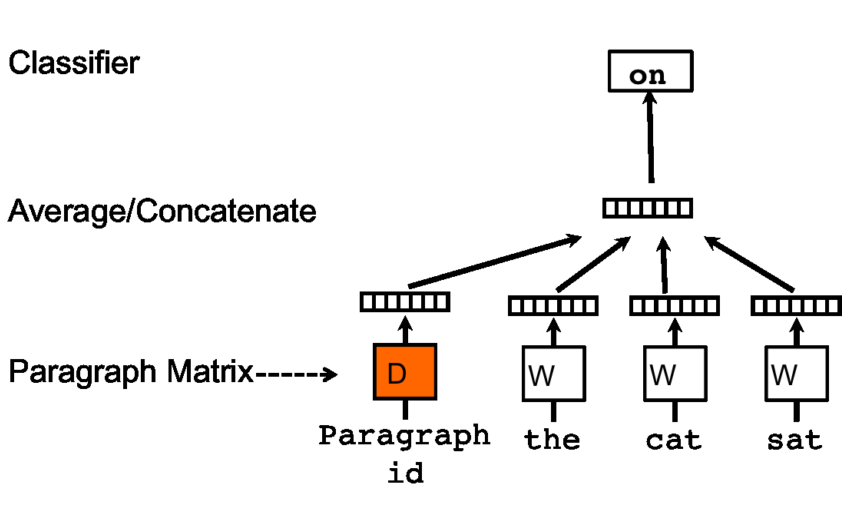
\includegraphics[width=0.7\linewidth]{le.png}
\caption{\texttt{word2vec} for paragraphs}
\label{fig:p2v}
\end{figure}
This paragraph representation could also be used for encouraging similarity between two bitext sentences.
In our novel approach, we will run the algorithm from \cite{Le2014}, but using the same paragraph vector when training word vectors from parallel sentences.
% is dat genoeg? of moet er iets bij over waarom we denken dat de alignments dan niet nodig zijn?
The sentence representation therefore acts as a way to relate the word spaces in both languages, without using word alignments.
% The method is general enough to allow training on more than two sentences. It also encodes more information in the vector than just bag-of-word-vector based models like Herman & Blunsum
We hope this will create a word vector space that is trainable on both monolingual and parallel data, allowing for the mitigation of sparsity in all languages.

% List of different models within this approach as discussed with Philip
We will explore at least two training methods:
\begin{itemize}
\item 
	Sequentially training all sentence pairs. As a paragraph id, we use a single identifier for every sentence pair in the bitext.
	This is equivalent to concatenating the parallel sentences and training from the context windows that do not bridge the sentence boundary.
\item 
	A two-step process:
	First creating paragraph representations for each sentence pair from a fully trained monolingual model. The information from the words in the first language will create a representation for the sentence.
	Then, we fix the sentence representations and train the word spaces in each language using these vectors.
	These sentence vectors will influence the learning of word embeddings in the other languages.
	The error gradient for the sentence vector can either be distributed over the words or be discarded.
\end{itemize}


\section{Experiments and evaluation}\label{s:experiments}

We are interested in comparing approaches to learn a word representation space for multiple languages. This vector space can be useful for a variety of tasks.


\paragraph{Training}

The source code is available for both \texttt{paragraph2vec}\footnote{Implemented as part of \url{https://github.com/piskvorky/gensim}} and \texttt{bicvm}\footnote{\url{https://github.com/karlmoritz/bicvm}}. The work in \cite{hermann2013multilingual} can be replicated with no further adjustments to \texttt{bicvm}.
Additionally, we should be able to train a vector space with more than two languages by tagging each word with a marker that specifies its language.
The new approach described above will need some small changes to \texttt{paragraph2vec}, but these are minimal.
We will implement and use the linear mapping algorithm described in section~\ref{s:lin} as a baseline.

As some of the methods require sentence-aligned (or word-aligned) data, we use the Europarl corpus for training. We hope to be able to use many languages, but at least three or four.
Possibly, Wikipedia or Reuters data can be used for extra monolingual training if needed.

% We'd like to combine the Europarl parallel sentences with the Wikipedia corpus in all 10 languages, to perform the joint learning of word embeddings from monolingual and bitext data.

\paragraph{Evaluation}




Both \cite{klementiev2012inducing} and \cite{hermann2013multilingual}
evaluate their methods on a real-world task: crosslingual document classification. The task is based on Reuters corpora, which has topic-annotated documents in English, French, German, Italian and Spanish. These languages are also in the Europarl data. Only documents that are assigned a single topic are used.

Each document is represented by the average of the representations of its tokens (in \cite{klementiev2012inducing}), or sentences (in \cite{hermann2013multilingual}).
An averaged version of the perceptron algorithm is trained for document classification in one language, and tested on data in another.
As a baseline, \cite{klementiev2012inducing} c
ompares to wordcount features. Translations are done via glossing or machine translation.

We use this same task and compute classification accuracy to compare the existing approaches described above to each other and to the new models introduced in \ref{s:newApproach}.


%In \cite{mikolov2013exploiting}, the evaluation is performed on a test set of gold-standard word translations, again from Google Translate. The word representation in the source language is transformed using $W$, and a ranked list of the nearest words in the target language is the output. The precision at ranks 1 and 5 is reported. 
% Gaan we dat nou ook nog doen of niet?

For visualizing the vector space, we will project a selection of words onto a plane and highlight semantic relationships.
We will also visualize rare words and words with high variability across languages.

\section{Deliverables}
We will write a 8-10 page ACL style research report on our findings. Furthermore, we will schedule a meeting with our supervisors and other
interested people. We will give an oral talk about our research and have a short discussion.

\bibliographystyle{plain}
\bibliography{bible}

\end{document}